\documentclass[sigconf]{acmart}

% Packages
\usepackage{makecell}
\usepackage{pifont}
\usepackage{float}
\usepackage{fontawesome5}
\usepackage{subcaption}
\usepackage{multirow}

% BibTex
\AtBeginDocument{%
  \providecommand\BibTeX{{%
    Bib\TeX}}}

% Copyright
\copyrightyear{2025}
\acmYear{2025}
\setcopyright{cc}
\setcctype{by}
\acmConference[ICAIF '25]{6th ACM International Conference on AI in Finance}{November 15--18, 2025}{Singapore, Singapore}
\acmBooktitle{6th ACM International Conference on AI in Finance (ICAIF '25), November 15--18, 2025, Singapore, Singapore}\acmDOI{10.1145/3768292.3770435}
\acmISBN{979-8-4007-2220-2/2025/11}

\settopmatter{printacmref=true}

% Document
\begin{document}

\title{Two Sides of the Same Coin: How LLMs Reveal Dual Narratives in Annual Reports}

\author{Xiao Li}
\authornote{Both authors contributed equally to the paper.}
\orcid{0009-0005-6418-2354}
\affiliation{
  \department{School of Computer Science}
  \institution{University College Dublin}
  \city{Dublin}
  \country{Ireland}}
\email{xiao.li@ucdconnect.ie}

\author{Changhong Jin}
\authornotemark[1]
\orcid{0000-0003-2565-592X}
\affiliation{
  \department{School of Computer Science}
  \institution{University College Dublin}
  \city{Dublin}
  \country{Ireland}}
\email{changhong.jin@ucd.ie}

\author{Yingjie Niu}
\orcid{0000-0001-9322-2726}
\affiliation{
  \department{School of Computer Science}
  \institution{University College Dublin}
  \city{Dublin}
  \country{Ireland}}
\email{yingjie.niu@ucdconnect.ie}

\author{Ruihai Dong}
\orcid{0000-0002-2509-1370}
\affiliation{
  \department{School of Computer Science}
  \institution{University College Dublin}
  \city{Dublin}
  \country{Ireland}}
\email{ruihai.dong@ucd.ie}

\renewcommand{\shortauthors}{Xiao Li, Changhong Jin, Yingjie Niu, and Ruihai Dong}

\begin{abstract}
   Annual reports (Form 10-K) are rich narrative documents, yet traditional textual analysis methods struggle to capture their deep semantic nuances and strategic positioning. This limitation is especially evident in the analysis of complex, multifaceted global events such as COVID-19. This study introduces a novel semantic scoring framework based on a Large Language Model (LLM) prompted with a Chain-of-Thought (CoT) reasoning process. The present framework has been developed for the purpose of quantifying the distinct narratives regarding the impact of the global events, and a firm's response within two critical sections of the 10-K: Item 1A (Risk Factors) and Item 7 (Management's Discussion \& Analysis, MD\&A). The core findings of this study highlight two key insights. Firstly, we propose a Dual Narrative Analysis framework, which enables to transform the scoring process into a transparent, verifiable analysis grounded in explicit evidence extraction from Item 1A and Item 7. Secondly, it is demonstrated that a Response Score extracted from the managerial narratives in Item 7 contains forward-looking information. A portfolio constructed based on this score has been shown to yield significant economic returns. The proposed methodology is both repeatable and expandable, and is intended to bridge the gap between disclosure and asset pricing.
\end{abstract}

\begin{CCSXML}
<ccs2012>
   <concept>
       <concept_id>10010147.10010178.10010179</concept_id>
       <concept_desc>Computing methodologies~Natural language processing</concept_desc>
       <concept_significance>500</concept_significance>
       </concept>
 </ccs2012>
\end{CCSXML}

\ccsdesc[500]{Computing methodologies~Natural language processing}

\keywords{10-K, Large Language Models, Chain-of-Thought, Financial NLP, Quantitative Text Analysis, Risk Quantification}

\maketitle

\section{Introduction}

The annual report (Form 10-K) required by the U.S. Securities and Exchange Commission (SEC) for public companies is not merely a compliance document, but rather a strategically designed narrative. The document under consideration includes audited quantitative financial data, as well as a large number of unaudited qualitative disclosures, the inclusion of which is at the discretion of management. 

These components are utilised by managers in the communication of information to stakeholders~\cite{healy2001information, loughran2016textual}, the management of impressions~\cite{brennan2022discretionary, leung2015impression}, and the indication of their perspective on the trajectory of the company in the future~\cite{call2024corporate}. This narrative component is a rich source of information, yet its value remains largely undiscovered~\cite{balakrishnan2010predictive}. A 10-K report is typically characterized by a high volume of text, which makes manual analysis at a large scale impractical~\cite{loughran2011liability, loughran2016textual, bassyouny2022narrative}.

Existing natural language processing (NLP) techniques employed in the financial domain exhibit non-ignored shortcomings in accurately interpreting complex narrative~\cite{loughran2016textual}. Early sentiment analysis approaches, including bag-of-words methods, dictionary-based models~\cite{loughran2011liability}, and readability assessments (e.g. the Fog Index~\cite{loughran2014measuring}), represented significant initial steps in the quantification of textual content.
However, these methods generally operate at a superficial level, capturing merely basic linguistic cues and largely ignoring the deeper, nuanced contexts that are crucial to meaningful financial interpretation~\cite{tang2025finmteb}.
Despite the evident potential of large language models (LLMs) in enhancing the quantitative analysis of financial texts, it is important to acknowledge the critical issues raised by LLMs. Analysts employ advanced comprehension capabilities of LLMs to assess the risks in annual reports~\cite{kothandapani2025ai, cao2024risklabs}. Nevertheless, the internal mechanisms and decision-making processes that generate these outputs remain entirely opaque~\cite{linardatos2020explainable}. 
The insights they provide are not capable of withstanding rigorous scrutiny or verification in high-risk financial environments~\cite{bender2021dangers}.

To address the above issue, we propose a \textbf{D}ual \textbf{N}arrative \textbf{A}nalysis (\textbf{DNA}) framework, which enables to constrain the analysis process of LLMs through structured prompting and Chain-of-Thought (CoT) reasoning. 
Specifically, in the proposed framework, the large language model (LLM) employed is not directly required to provide a final score. 
Indeed, the LLMs are instead used to guide the analysis of sections of the annual reports.
Firstly, the Impact Score is rated from Item 1A (Risk Factors) in order to quantify the potential severity of specific risks faced by the companies. 
Secondly, the Response Score is rated from Item 7 (MD\&A) in order to quantify the proactivity and quality of the management's response measures to the risk.

The LLM is guided through a series of predefined sub-tasks (i.e. identifying relevant paragraphs, judging content, and scoring based on evidence). 
Each score is accompanied by textual evidence of its source and a clear decision-making path, significantly enhancing the credibility and traceability of the results.
This approach provides a more comprehensive risk picture, enabling distinction between companies that are "high response" or "low response".
Furthermore, the Response Score applied to guide how to build portfolio strategies and validate their effectiveness in real-market conditions.
Our key contribution to the field include:

\begin{itemize}
    \item Through CoT reasoning, the model is guided to perform complex, structured semantic scoring, a technique which remains at the forefront of financial text analysis.
    \item By adapting the DNA framework to these distinct textual contexts, that is, one compliance-driven, and the other strategic-driven, deeper semantic insights are unlocked. 
    \item By empowering financial analysts and investors alike, the semantic insights enables to capture subtler signals embedded in corporate disclosures, and ultimately leads to more informed decision-making for portfolio investment.
\end{itemize}

\section{Related Work}

\subsection{Text analysis in the annual reports}

Financial text analysis has gained increasing attention in corporate risk identification and market impact research, especially as 10-K forms, providing official and authoritative information disclosure. 
In the early stages of the field, researchers relied on dictionary-based and statistical methods. 
For instance, the financial sentiment dictionary developed by Loughran and McDonald~\cite{loughran2011liability} effectively captured negative terminology, and the word frequency approach used by Hope et al.~\cite{hope2016benefits} measured corporate risk attitudes by tracking terms such as "risk" and "uncertainty".
However, these approaches have typically encountered challenges in processing context-dependent or ambiguous expressions, limiting their capacity to capture more subtly articulated forms.
As one of the earliest unsupervised topic modeling techniques, Latent Dirichlet allocation (LDA) has demonstrated practicality in revealing the underlying topic structure in financial text. 
Dyer, Lang, and Stice-Lawrence~\cite{dyer2017evolution} employed LDA to examine the longitudinal evolution of 10-K documents. 
Furthermore, Lopez-Lira~\cite{lopez2023risk} applied LDA to decompose the Item 1A of 10-K reports for textual interpretation and financial factor modeling. 
Although LDA provides an intuitive and computationally efficient method for the extraction of topics from financial text, the absence of contextual understanding limits its interpretability. 
This has prompted recent research to adopt more complex models, such as deep learning or LLMs.

The advent of deep learning has signified a paradigm shift in financial text analysis. 
For instance, Yang et al.~\cite{yang2020html} and Li et al.~\cite{li2024nlp} introduced a hierarchical Transformer-based model to capture multi-level semantics in 10-K disclosures that resulted in a significant improvement in stock volatility prediction.
Similarly, Backlund et al.~\cite{backlund2023detection} and Hu et al. \cite{hu2024zipzap} employ large pretrained language models, including BERT~\cite{devlin2019bert} and Longformer~\cite{beltagy2020longformer}, for tasks ranging from volatility forecasting to fraud detection and policy uncertainty modeling. 
Nevertheless, the modeling of extensive documents remains a significant challenge: conventional architectures commonly encounter token-length constraints, necessitating truncation or summarization, which in turn risks the omission of crucial semantic information. 
In addition, as Soong and Lin~\cite{soong2021sentiment} have observed, the structural elements of annual reports resulting in suboptimal identification of high-impact content.


\subsection{Risk Factors and MD\&A}

Recently, financial text analysis has increasingly emphasised the importance of section-specific narrative in annual reports, particularly two sections:

\begin{itemize}
    \item Item 1A (Risk Factors): This section explicitly requires companies to disclose material risks facing their operations. The primary objective is to promote transparency and caution, with the emphasis placed on delineating potential risks rather than expounding management responses or mitigation strategies. Consequently, its language is frequently formal, legalistic, and inherently conservative, thereby underscoring the seriousness and materiality of identified risks.
    \item Item 7 (MD\&A): This unaudited section allows company management considerable narrative freedom to present their perspective.  The MD\&A is crafted not only to inform but also to instill investor confidence, and thus typically adopts a proactive, explanatory, and forward-looking tone designed to highlight potential opportunities and strategic insights.
\end{itemize}

A number of studies have been conducted to explore the informational value and sentiment analysis of these sections.
Zhu et al.~\cite{zhu2024risk} demonstrated that, in the context of the financial crisis, the text in Item 1A of financial institutions became significantly more detailed and negative, and these changes are closely related to the actual risk experienced. 
Similarly, de Jong~\cite{de2025risk} examines the potential of Item 1A to serve as a leading indicator for future capital-raising events. 
From the perspective of investors, Kim et al.~\cite{kim2024learning} employ attention-based models to quantify the relative informativeness of different 10-K sections. They find that Item 7 consistently receives the most attention and contributes the majority to return prediction, closely followed by Item 1A.
Furthermore, Azmi Shabestari et al.~\cite{azmi2024textual} show that Item 7 has a significant effect on investor perception and valuation, whereas Item 1A has a weaker effect. 

\begin{figure*}[htbp]
    \centering
    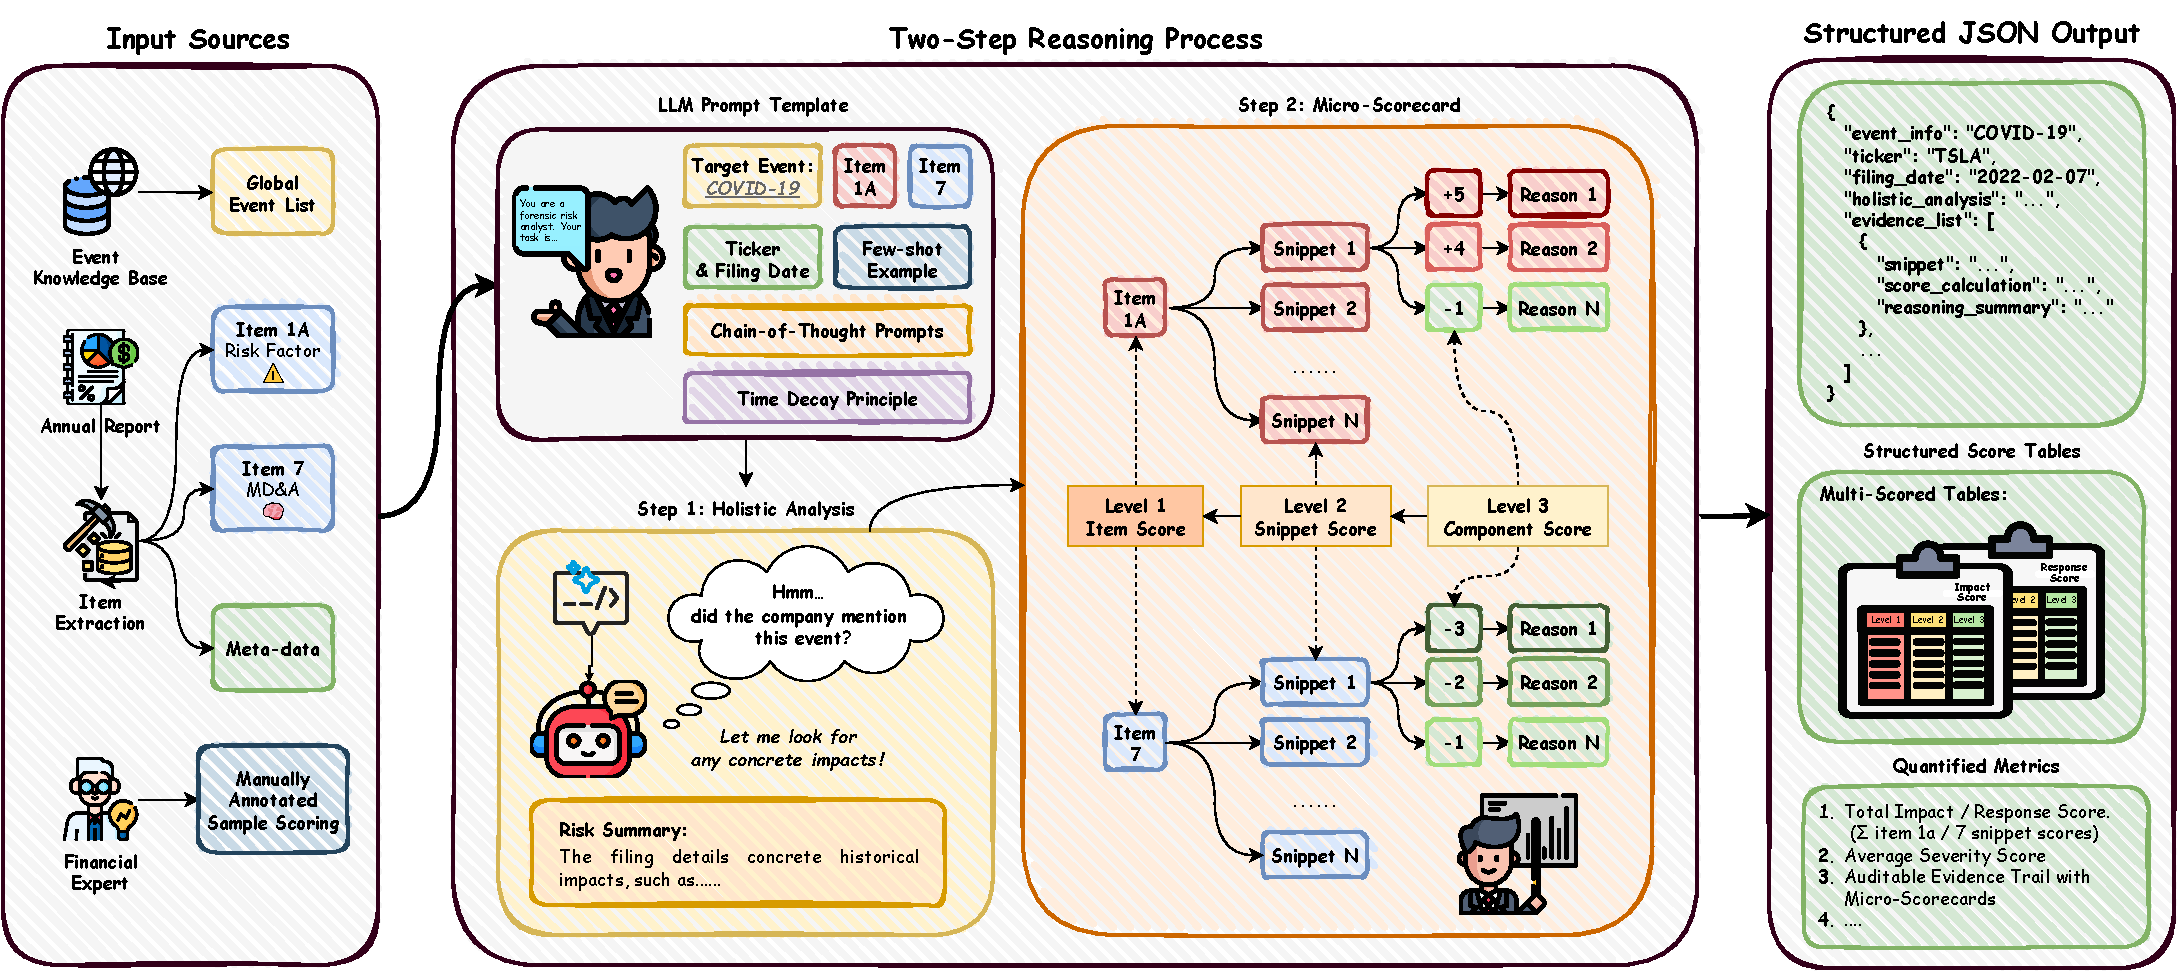
\includegraphics[width=\linewidth]{Figs/Framework.pdf}
    \caption{DNA Framework Using Chain-of-Thought (CoT) Reasoning for Quantifying Narratives on Global Events in Annual Reports (Form 10-K).}
    \label{fig:framework}
    \Description{}
\end{figure*}

\section{Methodology}

This study employs our DNA framework for measuring corporate risk exposure to specific global events as disclosed in annual reports. 
To achieve this objective, we introduce the "Chain-of-Thought Driven Micro-Scorecard Analysis" to transform the scoring process into a transparent, verifiable analysis grounded in explicit evidence extraction. 
Corporate risk narratives can be analyzed according to two independent and quantifiable dimensions.
The former is an \textit{Impact Score}, which is derived from the legally mandated disclosures in Item 1A (Risk Factors). 
The latter is a \textit{Response Score}, which captures the strategic managerial narrative presented in Item 7 (MD\&A). 
The analysis of these two dimensions independently enables the quantification of the "dual narrative" in corporate communication.

\subsection{Data and Corpus Construction}

Our study is based on three main types of data: (1) text data from corporate filings, (2) systematically selected global events, and (3) financial market data for portfolio construction and performance analysis, described further in Section~\ref{sec:portfolio}.

The text data consists of annual reports filed by S\&P 500 companies from 2021 to 2024~\cite{li2025flexibility}. We selected this period because many global events after 2020 significantly increased firm-level risk volatility, and we aim to examine how companies responded to these challenges. The filings were downloaded from the SEC EDGAR database\footnote{The SEC’s EDGAR database is available at \url{https://www.sec.gov/edgar}.}. Our DNA framework specifically focuses on two sections from each report: Item 1A (Risk Factors) and Item 7 (Management’s Discussion and Analysis, MD\&A). To ensure accurate metadata, we recorded each company's ticker symbol and filing date during the extraction process. This ensures a reliable link between our processed data and the original filings.

To connect our analysis to real-world events, we used significant global events identified through the Global Database of Events, Language, and Tone (GDELT)\footnote{The GDELT Project is available at \url{https://www.gdeltproject.org/}.}. From these events, we selected the \textit{COVID-19 pandemic} for detailed analysis, given its broad and significant impact on companies across various sectors.

To validate the risk scores derived from our text analysis, we collected financial market data from Yahoo Finance\footnote{Market data were retrieved using the \texttt{yfinance} Python package, available at \url{https://github.com/ranaroussi/yfinance}.}. Daily stock prices corresponding to each company’s fiscal year were collected. These data allowed us to calculate basic financial metrics, including stock returns for individual companies and stock index returns, helping us assess the predictive ability of our risk scores regarding real market performance.


\subsection{Dual Narrative Analysis Framework}

The architecture of the DNA framework is illustrated in Figure~\ref{fig:framework}, a Chain-of-Thought Driven Micro-Scorecard Analysis, transforming a general-purpose LLM into a specialized and auditable scoring engine. Unlike LLMs that directly score risk based on company and event information, our framework introduces three key innovations to address the challenges of controllability and transparency in quantitative text analysis:

\begin{enumerate}
    \item A multi-faceted prompt template that acts as a cognitive scaffold.
    \item A two-step reasoning process is required to ensure contextual depth.
    \item A strict separation between semantic analysis and final score computation.
\end{enumerate}

The process is initiated by our structured prompt template, which integrates five key components to create a rich, context-aware query for the LLM: the specific Target Event from our external knowledge base, Dynamic Context from the filing's metadata (Ticker, Filing Date), the full 10-K Item Contents, Few-Shot Examples to stabilize the output format, and a codified Time Decay Principle to enforce temporal logic. 

The assembled prompt then guides the LLM through a mandatory Two-Step Reasoning Process, which forms the core of the CoT reasoning.
Our core hypothesis is that forcing the LLM to first generate a comprehensive Holistic Analysis provides a stable, macro-level context that improves the quality and completeness of the subsequent micro-level analysis. Only after producing this narrative summary does the model proceed to the second step, Evidence Extraction \& Micro-Scorecard. Notably, this implementation represents a key component of the framework's innovation, specifically the dissection of all pertinent sentences and the subsequent allocation of positive or negative points to their constituent components, termed "Reasons." The hierarchical scoring process, in which reason-level points are aggregated to produce a snippet score, constitutes a key contribution to the transparency and verifiability of the LLM's reasoning.

Finally, our framework enforces a crucial separation of concerns. The LLM's role concludes with the generation of a Structured \textit{JSON} Output containing its detailed analytical components (the holistic analysis and micro-scorecards). The final aggregation into higher-level metrics, such as the Item Score Snippet Score, is deliberately offloaded to our programmatic backend. This design choice is a core part of our contribution to reproducible research, ensuring that the final Quantified Metrics are derived deterministically and are grounded entirely in the LLM's granular, auditable analysis.

\subsection{Risk Score Construction} 

The Micro-Scorecard employs a three-tiered scoring framework (see Figure~\ref{fig:framework}) to ensure the traceability and interpretability of the risk assessment process. First, at the Item level (Level 1), LLMs determine the corresponding Item category based on the labels of the input annual report content. Then, within each Item, the Micro-Scorecard further identifies text snippets (Snippet, Level 2) related to the target event. For each Snippet, the LLM decomposes the semantic content from multiple dimensions to generate the most granular Component scores (Level 3). Positive scores represent impacting factors, while negative scores represent mitigating factors or score deductions (such as deduction of losing description). All scores are synchronously recorded with their corresponding reason for further filtering.

All upper-level scores (Levels 1 and 2) follow a bottom-up aggregation strategy: first, Component scores are aggregated into Snippet scores, then into Item scores, and finally into upper-level scores. This hierarchical aggregation process retains detailed reason chains at each level, ensuring that the overall assessment system meets verifiability and audit requirements. Our backend integrates the scores based on Item type and score reasons to form finally multi-dimensional scoring metrics output.

\begin{figure}[htbp]
    \hypertarget{ex:risk_impact}{}
    \centering
    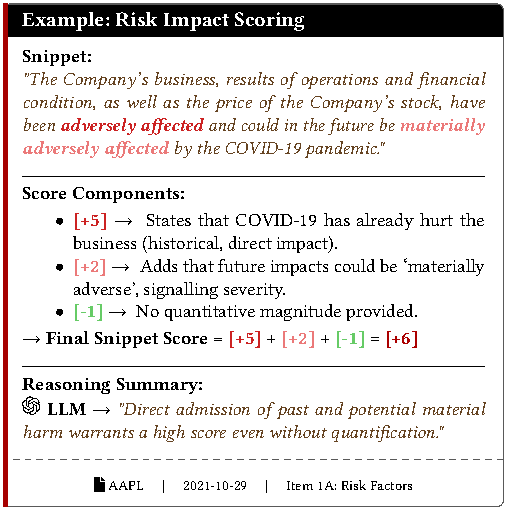
\includegraphics[width=\linewidth]{Figs/risk_impact_score.pdf}
    \Description{}
\end{figure}

\begin{figure}[htbp]
    \hypertarget{ex:risk_response}{}
    \centering
    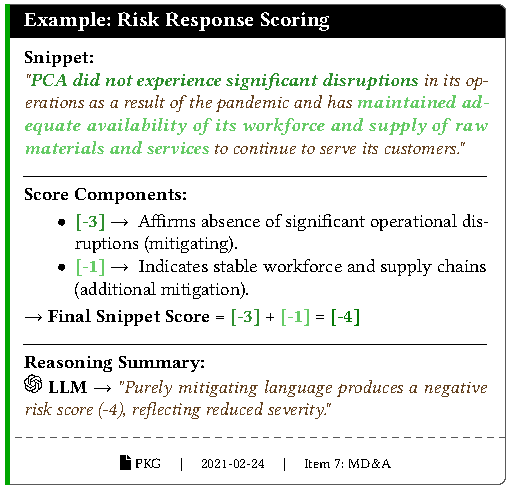
\includegraphics[width=\linewidth]{Figs/risk_responce_score.pdf}
    \Description{}
\end{figure}

Building upon this foundation, our framework constructs two distinct metrics for each event: a Impact Score (see \hyperlink{ex:risk_impact}{\textit{Example: Impact Score}}) and a Response Score (see \hyperlink{ex:risk_response}{\textit{Example: Response Score}}). The logical rationale for this dual-narrative structure is to disentangle the disclosure of risk perception from the discussion of managerial action. The Impact Score, derived from Item 1A, quantifies the magnitude of an event's potential negative consequences. A high positive score signifies a significant perceived adverse effect, driven by aggravating factors such as quantified potential losses. Conversely, the Response Score, derived from Item 7, quantifies the company's strategic reactions. Its interpretation is more nuanced: a high positive score indicates the narrative is still dominated by negative impacts, while a score near zero suggests a balanced discussion. Crucially, a negative score signifies a narrative predominantly focused on mitigating actions and countermeasures, as identified by the LLM through negative-point components in the micro-scorecards.

To ensure logical consistency, the entire scoring process is governed by our Time Decay Principle. This principle is grounded in the assumption that the acute perceived impact of most events diminishes over time, and it transforms this temporal logic into a set of hard constraints on the scoring process. The primary mechanism involves enforcing pre-defined scoring ceilings on a snippet's score based on the temporal distance between the event and the filing date. Evidence related to recent events (0-3 years) can receive high scores, while the maximum possible score for medium-term (4-10 years) and distant events (>10 years) is progressively reduced. This constraint is relaxed only when the text explicitly states a continuing or long-term impact. It is crucial to distinguish this rule-based temporal constraint from the semantically derived negative points that contribute to the Response Score. The distinction is made explicit within each micro-scorecard's reasoning, where a mitigating factor is attributed to textual evidence (e.g., "mentions a countermeasure"), whereas a temporal adjustment would be noted as a rule-based constraint on the final score.

To ensure logical consistency, the entire scoring process adheres to our Time Decay Principle. This principle is based on the assumption that the urgency perceived in most events diminishes over time, and translates this temporal logic into a series of hard constraints on the scoring process~\cite{chen2003life}. The main mechanism is to set predefined scoring caps for snippets based on the time interval between the event and the submission date. Evidence scores related to recent events (0–3 years) remain unaffected, while mid-term (4–10 years) and long-term events (>10 years) are subject to varying degrees of deductions based on the time span (with the lowest score being 0, used solely to weaken the Impact Score). This constraint is relaxed when terms such as "ongoing" or "long-term impact" appear in the Item content. Time decay deductions will appear as an independent component score in the county official snippet, along with a rationale, to facilitate filtering.

\subsection{Experimental Setup} 

The study is implemented in Python, which controls interactions with the OpenAI API. In particular, models from the \textit{GPT-o3} family are employed, since their performance on reasoning benchmarks is state-of-the-art, and in alignment with the two-step reasoning process embedded in the DNA framework.
The output of the DNA framework is driven by Chain-of-Thought–Driven Micro-Scorecard analysis.
The temperature parameter is fixed in all experiments, with the objective of maximising the determinism and reproducibility of the outputs. 
To ensure the reliability of the structured data extraction, we enforce the \textit{json\_object} response format in the API calls. The entire workflow is built upon the \textit{Langchain} library, which facilitates the dynamic prompt assembly, interaction with the LLM, and parsing of the structured outputs using \textit{Pydantic} models. The final aggregation of micro-scores into the Impact Score and Response Score is performed programmatically in our backend.

\begin{figure}[htbp]
    \centering
    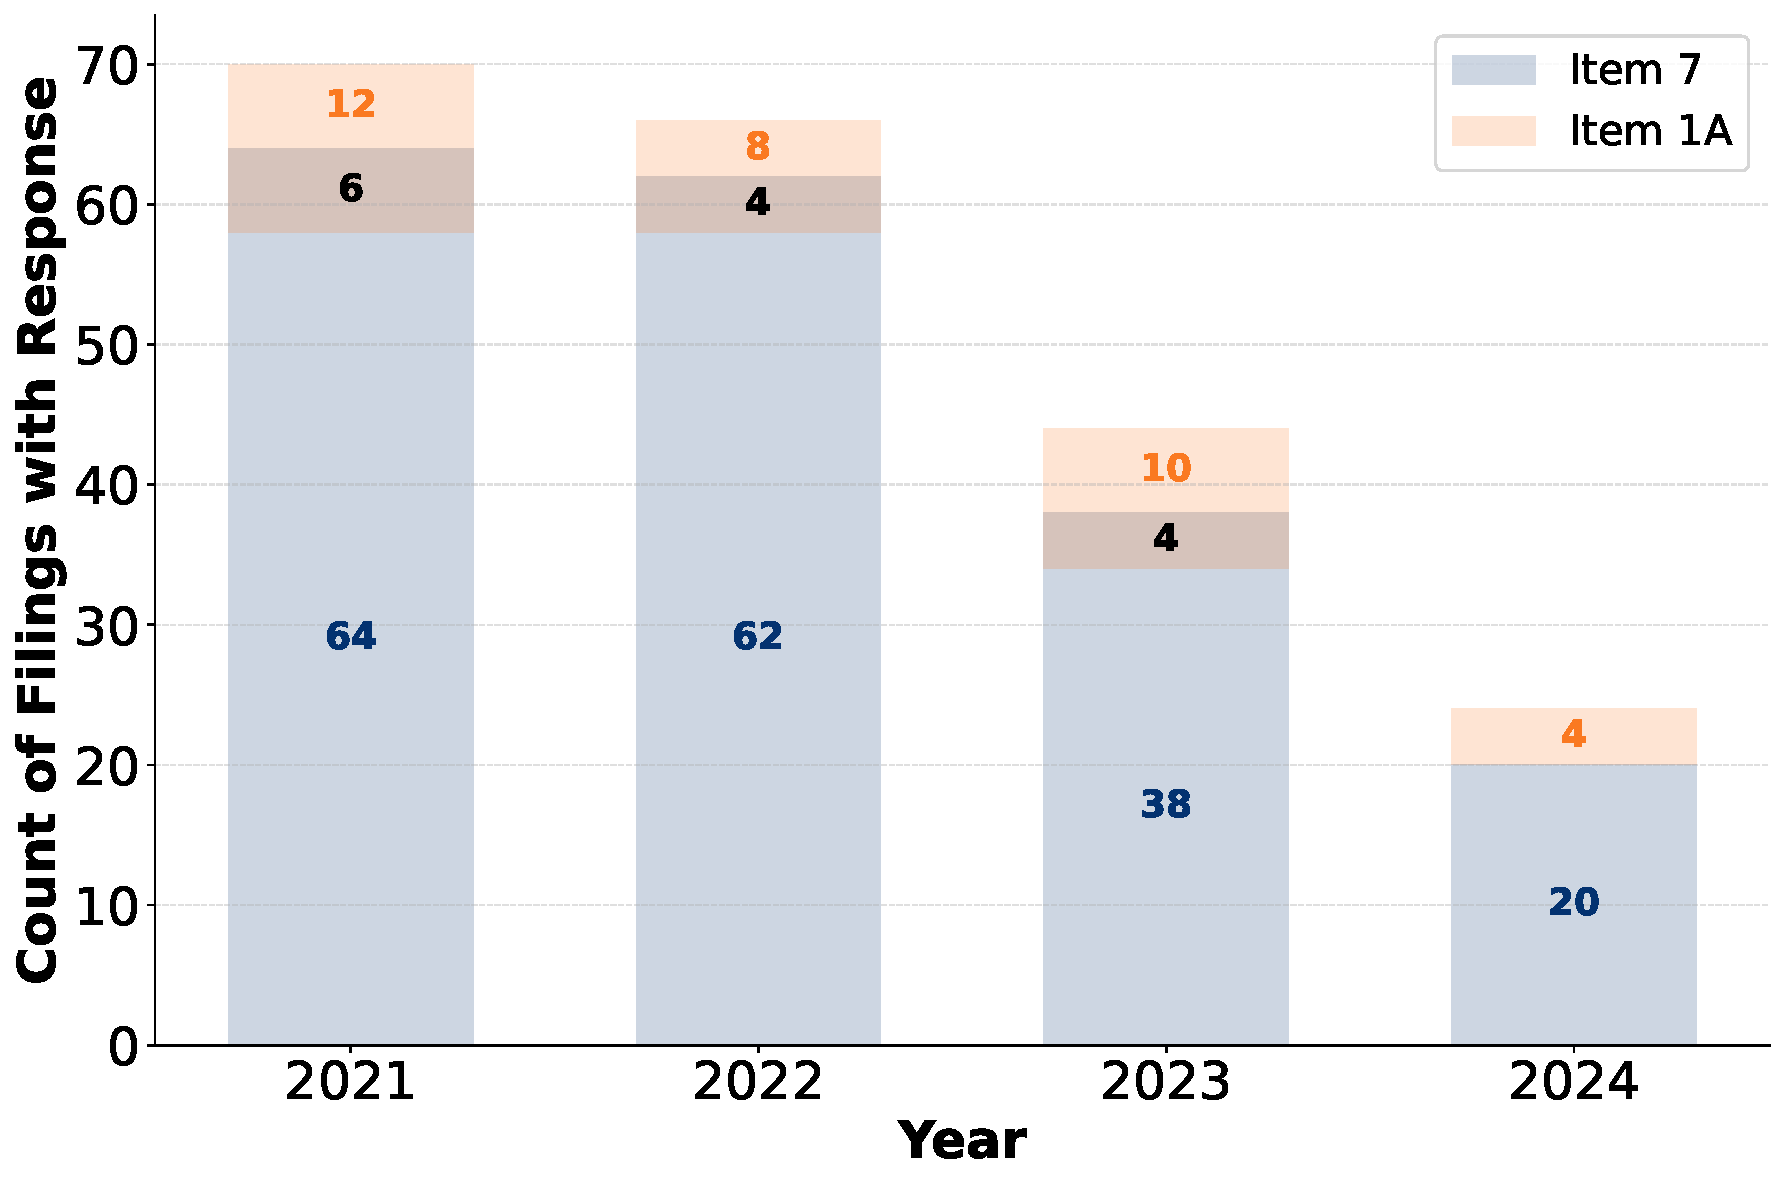
\includegraphics[width=\linewidth]{Figs/result_response_in_1a_7.pdf}
    \caption{The distribution of responsive snippets in items 1A and 7 in S\&P 500 10-K Filings (Submitted Date: 2021 – 2024).}
    \label{fig:distribution_response}
    \Description{}
\end{figure}

\section{Results and Discussion}

This section provides a detailed analysis and validation of the Impact Score and the Response Score. 
A key feature of the annual reports is the imbalance in the distribution of impact and response snippets. It is clear that firms place a greater emphasis on the disclosure of risks. This focus is affected by regulatory compliance requirements in Item 1A.
As demonstrated in Figure~\ref{fig:distribution_response}, the distribution of responsive snippets in items 1A and Item 7 is illustrated. The differences between the response snippets in the two sections are easily observed. 
However, in a small number of cases, companies also incorporate responsive narratives into Item 1A, or even distribute them across both sections. These observations indicate that firms may seek to project confidence by incorporating mitigation language into the risk disclosure. 
The imbalance and duplication of responsive narratives present a challenge in aligning the impact and response snippets in Item 1A and Item 7.
Furthermore, in view of the structural and semantic divergence, it is evident that Items 1A and 7 should be applied individually~\cite{azmi2024textual, kim2024learning}.

\subsection{Impact Score: Distribution and Trends}

The Impact Score aims to quantify the severity of the potential negative impact disclosed by the company in Item 1A that is triggered by a specific event. 
It is important to note that the annual reports are submitted between 2021 and 2024, and primarily describe events and financial performance in the previous fiscal year (i.e., 2020 to 2023).
As shown in Figure ~\ref{fig:violon_n_trend}, a visual analysis of the Impact Score for the 2020-2023 period was conducted.

\begin{figure*}[htbp]
  \centering
  \begin{subfigure}[t]{0.48\linewidth}
    \centering
    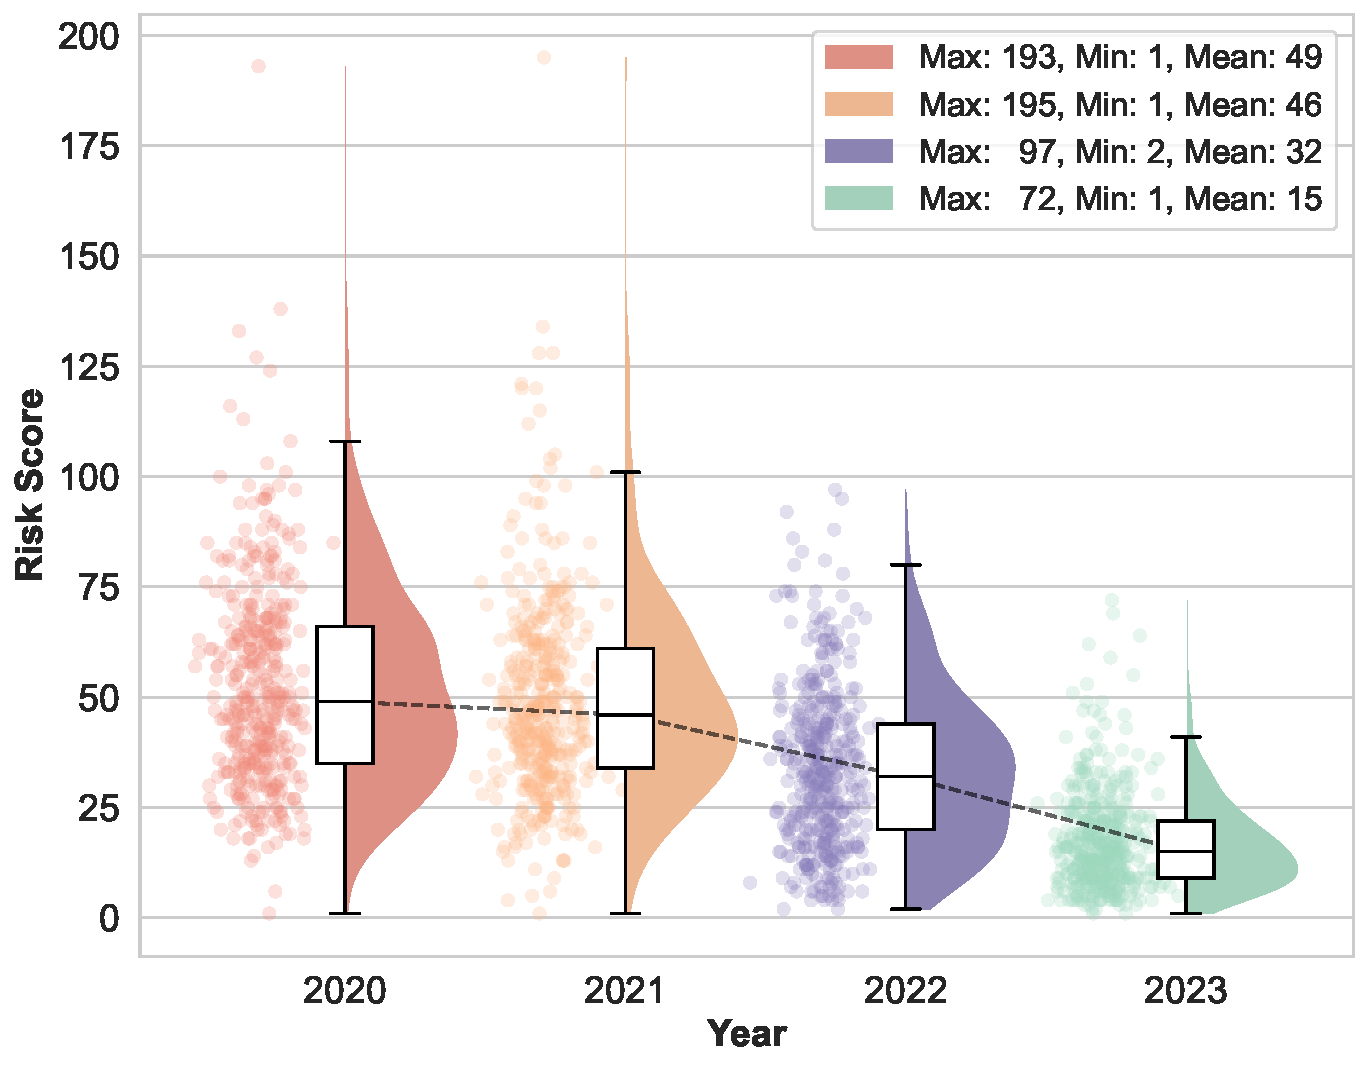
\includegraphics[width=\linewidth]{Figs/yearly_risk_trend_violin.pdf}
    \subcaption{}
    \Description{violin plot}
  \end{subfigure}\hfill
  \begin{subfigure}[t]{0.48\linewidth}
    \centering
    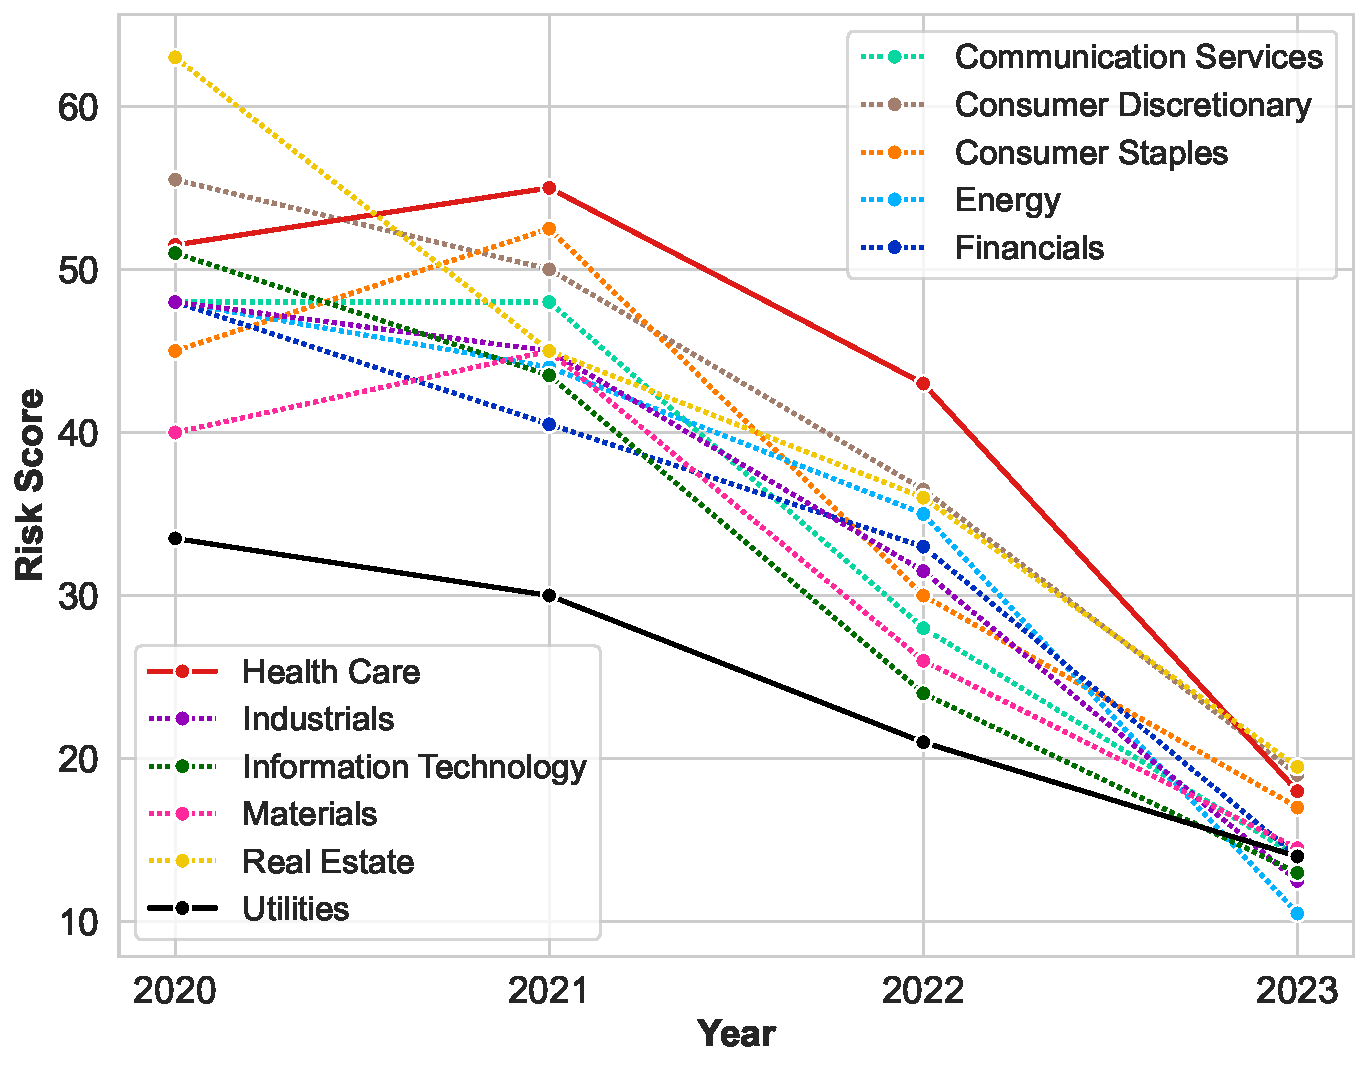
\includegraphics[width=\linewidth]{Figs/yearly_risk_trend_avg.pdf}
    \subcaption{}
    \Description{trend plot}
  \end{subfigure}
  \caption{Evolution of Firm-Level Impact Scores (2020 – 2023). (a) yearly score distributions across all S\&P 500 firms. (b) yearly mean scores by GICS sector.}\label{fig:violon_n_trend}
\end{figure*}

The violin plot indicates a consistent year-on-year decrease in the mean value of the Impact Score, accompanied by a notable reduction in the standard deviation of the scores.
Specifically, During the initial phase of the COVID-19 pandemic (2020–2021), risk perceptions exhibited significant variation across firms, as evidenced by the broad distribution of scores. This observed heterogeneity is attributable to the uneven and unpredictable nature of the pandemic's impact across diverse industry sectors and geographical regions.
Since 2022, there has been a tendency for the Impact Score to converge, reflecting not only an overall decrease in perceived risk but also an increasing convergence among companies in the manner in which they present and construct external threats. This convergence indicates a collective shift towards post-COVID-19 normalisation, whereby companies adopt more standardised language to describe recurring or stabilised risks.

Furthermore, sector-level trends, as outlined in the Global Industry Classification Standard (GICS), serve to highlight the heterogeneous evolution of pandemic-related risk narratives. In the initial phases, elevated risk scores were particularly concentrated in sectors such as real estate, consumer discretionary, and healthcare, which were directly exposed to physical restrictions, demand shocks, and public health uncertainties.
By 2023, the utilities sector consistently exhibited the lowest risk scores, reflecting its relative insulation from pandemic-induced volatility due to regulated revenue streams and its status as an essential service. In contrast, the healthcare sector exhibited sustained elevated risk levels, highlighting the extended uncertainties surrounding regulatory dynamics, supply chain constraints, and evolving public health risks.

\subsection{Response Score: Interpretation and Validity}

The response score aims to quantify the intensity of the company's discussion of its strategic response measures and risk mitigation strategies in Item 7. For this purpose, we build a case table, as shown in Table~\ref{tab:scorecard-response}), which lists the scoring range and corresponding specific narrative patterns.

It was observed that approximately 85\% of the snippets obtained positive scores (i.e. $>0$), with the narrative remaining firmly focused on the negative impacts of the event, even in the sections of Item 7, which primarily reflected the operational challenges posed by the event rather than mitigation strategies. 
This phenomenon underscores the tendency for management discussions to accentuate negative impacts. Snippets with a score of 0 account for approximately 4\% of the total analysis, corresponding to neutral statements that vaguely mention the event's impact without providing any specific details or mitigation measures.
It is noteworthy that within the negative score range, approximately 11\% of snippets have scores below 0. 
To further refine the classification, the negative-value samples were divided into two intervals based on their distribution: The top 50\% distribution (e.g., $-2.5$ or less) is indicative of a strong mitigation strategy, frequently accompanied by explicit negative descriptions, such as explicit statements that the event has no material impact on financial performance, or the provision of clear details of mitigation responses. 
The lower 50\% interval ($-2.5$ to $0$) indicates weaker mitigation strategies, commonly observed in responses to external macroeconomic factors (e.g., interest rates or policies) where the response is ambiguous.

\section{Risk-Response-Driven Portfolio Strategy}
\label{sec:portfolio}

This study is prompted by an anomaly that has been empirically validated: companies that voluntarily disclose risk response measures in Item 7 of their MD\&A in Form 10-K reports exhibit significantly higher cumulative excess returns than their non-disclosing peers over the long term. Previous studies have shown that the forward-looking information in the MD\&A has predictive value for firm performance and market returns \cite{li2010information, loughran2011liability}. However, there are two possible reasons why a company might choose not to disclose information: (1) the risks it faces are extremely low and do not warrant mention, or (2) the risks are not low, but the company chooses not to disclose them in order to play down the risks, or because it has no response measures in place. 

\begin{table*}[t]
  \centering
  \small
  \caption{Interpretation Framework for the Risk Response}
  \label{tab:scorecard-response}
  \setlength{\tabcolsep}{3pt}
  \resizebox{\textwidth}{!}{
    \begin{tabular}{c c c p{6.9cm} p{6.1cm}}
      \toprule
      \textbf{Score Range} &
      \textbf{Response Level} &
      \textbf{Sample Score$^{\dagger}$} &
      \textbf{Example Snippet} &
      \textbf{Rationale / Interpretation} \\
      \midrule

      \multirow{4}{*}{$\le -2.5$} &
      \multirow{4}{*}{\textit{Significant Mitigation}} &
      \multirow{4}{*}{-4} &
      "We have ... \textbf{enabled employees to work from home} ...; \textbf{adjusted work spaces} and \textbf{shift schedules} ...; \textbf{required face coverings} and \textbf{distributed personal protective equipment (PPE)}." &
      Extensive operational mitigation: covers remote work, on-site protocols, sanitation, and PPE—indicating a comprehensive COVID-19 response. \\
      \midrule

      \multirow{4}{*}{$(-2.5, 0)$} &
      \multirow{4}{*}{\textit{Partial Mitigation}} &
      \multirow{4}{*}{-2} &
      "In addition, when negative economic conditions have been particularly severe, like during the Covid-19 pandemic, we have moved decisively to \textbf{lower operating expenses} to improve financial performance." &
      Suggests a mitigating response through cost reduction, but the absence of concrete measures or operational details limits the strength of evidence—warranting a moderate mitigation score of $-2$. \\
      \midrule

      \multirow{3}{*}{0} &
      \multirow{3}{*}{\textit{Neutral / Indeterminate}} &
      \multirow{3}{*}{0} &
      "We continued to see the commercial aerospace end market recover from the COVID-19 pandemic and were encouraged by the progress of the commercial aerospace market recovery." &
      Not actively mitigated, but partially mitigated by market recovery. \\
      \midrule

      \multirow{3}{*}{$> 0$} &
      \multirow{3}{*}{\textit{No Mitigation}} &
      \multirow{3}{*}{3} &
      "Certain of the Company’s \textbf{component suppliers} and \textbf{logistical service providers} experienced \textbf{disruptions}, resulting in \textbf{supply shortages} that affected sales worldwide." &
      Explicit link to worldwide sales impact (supply shortage). \\
      \bottomrule
    \end{tabular}
  }

  {\footnotesize \textit{Note.} $^{\dagger}$ The \emph{Sample Score} column shows one representative component selected from the full Micro-Card assigned to the highlighted snippet.}
\end{table*}



To distinguish between these, we use our Impact Score measure from Item 1A (Risk Factors) to quantify objective risk exposure. The results (Figure~\ref{fig:violon_n_trend}) show that all sample companies, across all industries and years, face significant risks. This rules out the 'no-risk' assumption and suggests that companies that are willing to disclose their responses are more likely to have transparent and mature risk management systems. Conversely, those that remain silent may have motives to reduce the visibility of risks. Based on this logic, we propose the core hypothesis that a portfolio composed of companies with abundant responses should systematically outperform a portfolio composed of companies with missing responses in terms of risk-adjusted returns. The remainder of this section rigorously tests this hypothesis through backtesting.

\subsection{Portfolio Construction Methodology}

To construct an empirical setup capable of effectively testing our hypotheses, we adopt the portfolio backtesting method widely used in academic financial research using stocks from the S\&P 500 Index, with a particular focus on avoiding "Look-Ahead Bias".

To strictly simulate real-world investment decisions and avoid look-ahead bias, we have adopted the common time frame used in financial academic research \cite{fama1993common, carhart1997persistence, cooper2008asset, hou2015digesting}. Under this framework, annual reports (10-K) describing the situation in year $t-1$ are considered to have been published by \textit{30th June} of year $t$. Based on this, we set \textit{1st July} of each year as the date for portfolio construction or rebalancing to ensure that all decisions are based on information that was fully disclosed as of the previous day. The constructed portfolio is held for one year, until \textit{30th June} of the following year. This one-year holding period aligns with the annual report analysis cycle, aiming to test the validity of the text signal over the medium term.

On each year’s rebalancing date (\textit{1st July}), we first identify all S\&P 500 constituents that have released their most recent annual reports. We then sort these firms in descending order by their model–estimated \emph{Response Score} $S_{i,t}$, where $i$ indexes the firm and $t$ denotes the rebalancing year. 
Inspired by Niu et al.~\cite{niu2024evaluating}, we construct two highly differentiated portfolios based on the ranking:

\begin{enumerate}
    \item \textbf{With Response Portfolio} ($P_{response}$): The portfolio consists of the 20 companies with the lowest scores (i.e., their Response Scores are negative, indicating that they have taken measures to address the risks).
    \begin{equation}
        P_{response, t} = \{i \mid \text{rank}(S_{i,t}) \le 20 \text{ and } S_{i,t} < 0\}
    \end{equation}
    \item \textbf{Without Response Portfolio ($P_{no\_response}$)}: The portfolio consists of the 20 companies with the highest scores (i.e., their Response Scores are positive or zero, indicating no response measures).
    \begin{equation}
        P_{no\_response, t} = \{i \mid \text{rank}(S_{i,t}) > N-20 \text{ and } S_{i,t} \geq 0\}
    \end{equation}
    Where $N$ is the total number of companies with available scores for that year.
\end{enumerate}

Within each of the two investment portfolios, all constituent stocks are allocated using an equal weighting approach. We chose equal weighting over market capitalization weighting primarily to eliminate the excessive influence of large-cap stocks on portfolio performance. If market capitalization weighting were used, the portfolio's returns could be dominated by the performance of a few large companies, thereby masking the predictive power of our "risk response bias" score itself. The equal weighting method ensures that each selected company's signal contributes equally to the overall performance of the portfolio.

\subsection{Performance Evaluation Metrics}

We use daily cumulative return as the core evaluation indicator because it intuitively reflects the capital appreciation process of investors throughout the backtesting period. For an investment portfolio $P$, the cumulative return $CR_T$ from the start of backtesting ($d=0$) to day $T$ is calculated as follows:
\begin{equation}
    CR_T = \prod_{d=1}^{T} (1 + R_{P,d})-1 \quad \text{where} \quad R_{P,d} = \frac{1}{K} \sum_{i \in P} R_{i,d}
\end{equation}

In this formula, $K$ = 20 is the number of companies in the portfolio, and $R_{i,d}$ is the return of company $i$ on day $d$.

In addition to the cumulative yield curve, we have introduced the Sharpe Ratio and Maximum Drawdown as supplementary risk-adjusted return metrics for a more comprehensive assessment.

\subsection{Empirical Results and Discussion}

Our backtesting covers a 4 year period from \textit{July 1, 2021}, to \textit{June 30, 2025}, and the results provide strong empirical support for our core assumptions. As shown in Figure~\ref{fig:portfolio_cumulative} and Table~\ref{tab:portfolio_result}, the most important finding is the significant performance divergence between the "responsive group" and the "non-responsive group". The "responsive group" not only consistently outperformed the "non-responsive group" in cumulative returns but also demonstrated a decisive advantage in key performance metrics: its annualized return rate (13.78\%) was more than three times that of the "non-responsive group" (3.75\%), while its Sharpe ratio (0.75) was significantly higher than the latter's 0.23, indicating superior risk-adjusted returns. This result directly validates our core hypothesis that a lower Response Score can effectively distinguish companies with superior future performance.



\begin{table}[t]
\centering
\setlength{\tabcolsep}{3pt}
\renewcommand{\arraystretch}{1.2}
\caption{Key Performance Metrics of Portfolios}
\resizebox{\linewidth}{!}{
\begin{tabular}{lccc}
\toprule
\textbf{Metric} & \textbf{With Response} & \textbf{Without Response} & \textbf{S\&P 500} \\
\midrule
Annualized Return           & 13.78\%   & 3.75\%    & 10.72\%   \\
Annualized Volatility       & 18.28\%   & 16.25\%   & 17.38\%   \\
Sharpe Ratio                & 0.75      & 0.23      & 0.62      \\
Max Drawdown                & -22.15\%  & -22.84\%  & -20.02\%  \\
\bottomrule
\end{tabular}}
\label{tab:portfolio_result}
\end{table}

In comparison with the market benchmark, S\&P 500, the efficacy of the strategy under consideration has also been demonstrated. The "responsive group" not only outperformed the S\&P 500 in absolute returns (13.78\% vs. 10.72\%), but also outperformed it in Sharpe ratio (0.75 vs. 0.62), meaning that our strategy delivered higher returns while taking on similar levels of risk.
Additionally, its maximum drawdown (-22.15\%) was better than the "non-responsive group" (-22.84\%), demonstrating greater resilience in extreme market conditions. 
However, its drawdown was still higher than the S\&P 500 (-20.02\%), which may be due to the relatively concentrated portfolio (20 stocks) resulting in higher individual stock-specific risks compared to the highly diversified market index. 

The economic intuition behind these empirical results is clear. Firstly, the act of proactively disclosing risk response measures is itself a positive signal. It conveys to the market that management has control over the company's operations and is accountable to shareholders, thereby reducing information asymmetry and boosting investor confidence \cite{healy2001information}. Secondly, such disclosure behavior is typically associated with stronger corporate governance and more robust internal risk management frameworks \cite{eng2003corporate, kim2024learning}. Companies with these superior fundamentals demonstrate greater operational resilience in the face of macroeconomic headwinds, thereby providing support for their stock prices.

In summary, the findings of this case study reveal that capital markets exhibit pricing lag in response to qualitative risk management information disclosed in annual reports. By quantifying "risk response", we successfully captured this market inefficiency, demonstrating the signal's effectiveness in generating excess returns and providing investors with a new perspective beyond traditional financial metrics.

\balance

\section{Conclusion}

This study presents a DNA framework that uses large language models (LLMs) and Chains of Thought (CoTs) to analyse the narrative analysis of companies' 10-K reports in depth. Our core contributions are as follows: firstly, we present a novel  technique for quantifying and interpreting the underlying narratives of companies. We demonstrate its validity by revealing the dual narrative structure between Item 1A (Risk Factors) and Item 7 (MD\&A). Secondly, we demonstrate that the narrative analysis can create real economic value for investors, as the Response Scores rated from management's narrative snippets can be used for portfolio strategy.

\begin{figure}[tbp]
    \centering
    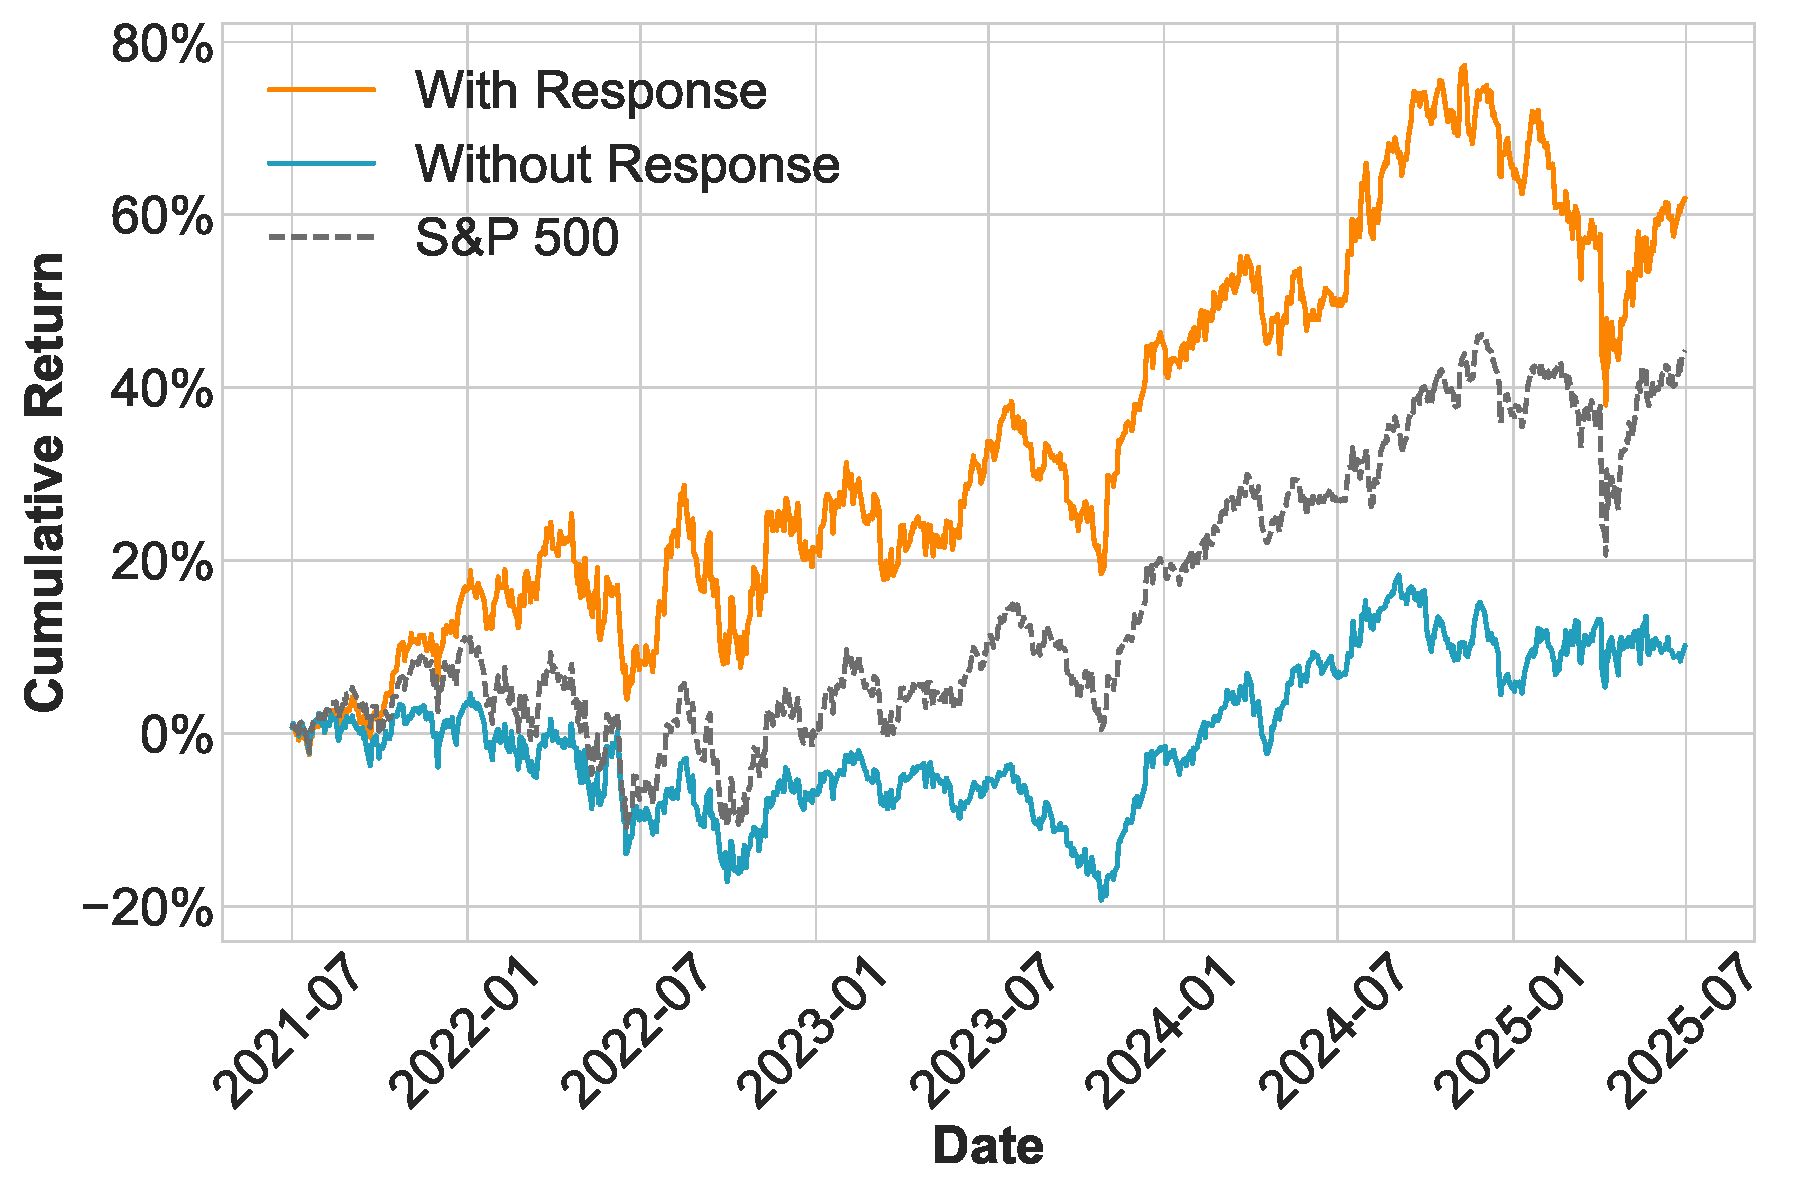
\includegraphics[width=\linewidth]{Figs/portfolio_cumulative_returns_action_vs_no_action.pdf}
    \caption{Portfolio Cumulative Returns, Action vs No Action (with baseline S\&P 500)}
    \Description{Portfolio Cumulative Returns, Response VS No Response}
    \label{fig:portfolio_cumulative}
\end{figure}

While the present implementation employs the Impact Score for Item 1A and the Response Score for Item 7, the potential value of integrating these two scores would be recognised. In future work, we plan to explore joint modeling strategies that combine them framing into a unified narrative trajectory. 

\begin{acks}
This research was conducted with the financial support of Research Ireland [12/RC/2289\_P2], at the Insight Research Ireland Centre for Data Analytics at University College Dublin. The study also gratefully acknowledges financial support from the China Scholarship Council (CSC), which played a crucial role in supporting the researcher’s development and facilitating international collaboration.
\end{acks}

\bibliographystyle{ACM-Reference-Format}
\bibliography{ref}

\end{document}